\section{Remove recent apps button from navigation bar. E.g.:  App custom navigation bar}\label{sec:ch6}
\subsection{Introduction}
This assumes you just did a fresh install of LineageOS osprey 14.1 nightly build.
\subsection{Steps:}
\begin{enumerate}
    \item download fdroid
    \item download terminal emulator from fdroid
    \item download custom navigation bar from an alternative source such as: \url{https://www.apkmirror.com/apk/paphonb/custom-navigation-bar/custom-navigation-bar-0-8-11b-release/custom-navigation-bar-0-8-11b-android-apk-download/download/}
    \item rename it to customNavBar.apk, install it. (it was named: \url{xyz.paphonb.systemuituner_0.8.11b-118_minAPI24(nodpi)_apkmirror.com.apk} with command:
\begin{verbatim}
adb install customNavBar.apk
\end{verbatim}
    \item Then give custom navigation bar root access from adb with command:
\begin{verbatim}
adb shell pm grant xyz.paphonb.systemuituner android.permission.WRITE_SECURE_SETTINGS    
\end{verbatim}
    \item once that is done, ignore the next command you are supposed to enter in the android terminal emulator listed below. (I entered it several times but it kept saying I should grant runtime access. That is done with the adb command above. After the adb command above I did not re-enter the command below. (But just in case it did influence the procedure here it is):
\begin{verbatim}
pm grant xyz.paphonb.systemuituner android.permission.WRITE_SECURE_SETTINGS    
\end{verbatim}
    \item Then open the custom Navigation bar app.
    \item do the compatibility test. It should change the home button to the little arrow shown in the middle of \cref{fig:diag}.
    
    \begin{figure}[H]
        \centering
        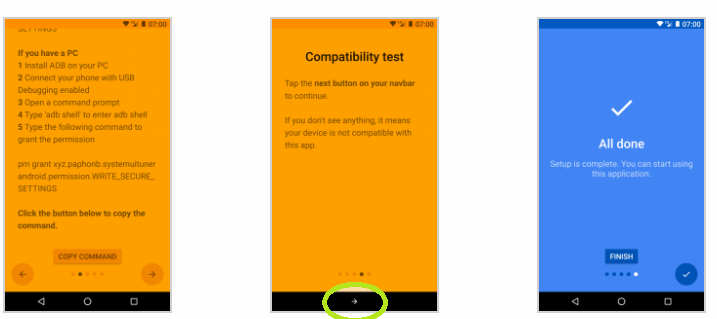
\includegraphics{images/pic.png}
        \caption{If the custom navigation app works with your phone the diagnostic test should change the home button as shown in the green circle.}
        \label{fig:diag}
    \end{figure}
    \item Next, in the app click "experimental features" and remap the "overview " button to "home".
    \item that's it. Now quickly reboot and uninstall the app as it shared your data. (The remapping will remain active after de-installation!
\end{enumerate}